\chapter{相对论动力学}\label{ch:b3:relativistic-dynamics}

1964 年，威廉·伯托齐拍下了电子在直线
加速器中飞驰的情景：每一束电子都被赋予一个测得的能量，其速率
则在 \qty{8.4}{m} 的飞行距离上计时。牛顿预言，
\qty{15}{MeV} 的电子应以光速的八倍飞行；
秒表却显示 $0.9999c$，此后不肯再增长，无论
如何推动电子。运动学在上一章已指出，$c$ 是速率的上限；
动力学现在必须解释推力的去向——
即速率不再增长时，功去了何处。答案是，
力学需围绕新的动量与新的能量重组，二者统一于
物理学中最著名的方程：储存的能量即质量，质量即驻留的能量，
$E = mc^2$。本章建立这一动力学，
并将其用于它日常所在之处：放射性衰变、
粒子碰撞，
以及把运动转化为新物质的加速器。

\section{动量与能量的重建}

\begin{remark}[为何要舍弃 $m\vect v$]\label{rem:b3:relativistic-dynamics:why}
经典动量 $m\vect v$ 在每个参考系中均守恒，\emph{前提是}
速度按伽利略方式变换。事实上并非如此
（见\cref{prop:b3:relativistic-kinematics:addition}）：一次碰撞若在一个参考系中守恒
$\sum m\vect v$，在另一参考系中便不再守恒，因此旧动量
不能作为自然定律——至多只是低速时的
影子。修正之法在于以
粒子\emph{自身}的时钟来测量速度：$\dd\vect r/\dd\tau =
\gamma\,\vect v$ 变换得十分干净，而 $m\,\dd\vect r/\dd\tau$ 结果
却在所有参考系中同时守恒。
\end{remark}

\begin{definition}[相对论动量与能量]\label{def:b3:relativistic-dynamics:momentum-energy}
\index{相对论动量}\index{相对论能量}\index{静能}
质量为 $m$、速度为 $\vect v$ 的粒子（$\gamma = 1/\sqrt{1 -
v^2/c^2}$）具有动量与能量
\[
\vect p = \gamma m\vect v , \qquad
E = \gamma mc^2 .
\]
静止时 $E_0 = mc^2$：即\emph{静能}。动能则是运动所增加的
部分，$E_k = E - mc^2 = (\gamma - 1)mc^2$；当 $v
\ll c$ 时，约化为熟悉的 $\tfrac12 mv^2$（展开 $\gamma$ 即可）。
在每个孤立过程中，总动量 $\vect p$ 与总能量 $E$——包括静能
在内——均守恒。
\end{definition}

\begin{theorem}[能量–动量关系]\label{thm:b3:relativistic-dynamics:relation}
\index{能量–动量关系}
对任一粒子，
\[
E^2 = (pc)^2 + (mc^2)^2 ,
\qquad
\vect v = \frac{\vect p\,c^2}{E} :
\]
组合 $E^2 - p^2c^2 = m^2c^4$ 在各
参考系中取值相同——它之于能量与动量，恰如\omterm{thm:b3:relativistic-kinematics:interval}{时空间隔}之于时间与
空间。两种情形：低速时，$E \approx mc^2 + p^2/2m$；在
高能（$E \gg mc^2$）时，$E \approx pc$ 且 $v \to c$：加大推力，
只增加能量与动量，几乎不增加速率。
\end{theorem}

\begin{proof}
$E^2 - p^2c^2 = \gamma^2m^2c^4(1 - v^2/c^2) = m^2c^4$；又 $pc^2/E =
\gamma mvc^2/\gamma mc^2 = v$。参考系不变性之所以成立，是因为 $m$
和 $c$ 均与参考系无关。
\end{proof}

\begin{proposition}[无质量粒子]\label{prop:b3:relativistic-dynamics:massless}
\index{光子!动量}
质量为零的粒子有 $E = pc$，且在每个
参考系中都恰以速率 $c$ 运动；它不能被减速，只能产生红移。光子便是
典型例子：$E = h\nu$ 与 $p = h\nu/c = h/\lambda$——即
本科一年级分册中的普朗克–爱因斯坦关系，如今可视作
力学中 $m = 0$ 的特例。
\end{proposition}

\begin{proof}
在\cref{thm:b3:relativistic-dynamics:relation}中令 $m = 0$，得 $E = pc$
且 $v = pc^2/E = c$。
\end{proof}

\begin{omfigure}
\begin{tikzpicture}
  \begin{axis}[omaxis, axis x line=bottom, axis y line=left,
    width=6.6cm, height=5.4cm, xmin=0, xmax=4.3, ymin=0, ymax=1.35,
    xlabel={$E_k/mc^2$}, ylabel={$v^2/c^2$},
    xlabel style={at={(axis description cs:0.5,-0.1)}, anchor=north},
    xtick={1,2,3,4}, ytick={0.5,1}, clip=false]
    \addplot[omExo, dashed, thick, domain=0:0.68] {2*x};
    \addplot[omDef, very thick, domain=0:4.3, samples=80] {1 - 1/(1+x)^2};
    \addplot[gray, dashed, domain=0:4.3] {1};
    \node[omExo, font=\scriptsize, anchor=west] at (axis cs:0.8,1.24) {牛顿：$v^2 = 2E_k/m$};
    \node[omDef, font=\scriptsize, anchor=west] at (axis cs:2.0,0.82) {相对论};
    \fill[omThm] (axis cs:0.87,0.714) circle (1.6pt);
    \fill[omThm] (axis cs:1.96,0.886) circle (1.6pt);
    \fill[omThm] (axis cs:2.94,0.935) circle (1.6pt);
  \end{axis}
  \begin{axis}[omaxis, axis x line=bottom, axis y line=left,
    width=6.6cm, height=5.4cm, xmin=0, xmax=3, ymin=0, ymax=3.3,
    xshift=7.2cm,
    xlabel={$pc/mc^2$}, ylabel={$E/mc^2$},
    xlabel style={at={(axis description cs:0.5,-0.1)}, anchor=north},
    xtick={1,2,3}, ytick={1,2,3}, clip=false]
    \addplot[omDef, very thick, domain=0:3, samples=60] {sqrt(1+x*x)};
    \addplot[omExo, dashed, domain=0:3] {x};
    \draw[<->, omThm] (axis cs:0,0.04) -- (axis cs:0,0.96);
    \node[omThm, font=\scriptsize, anchor=west] at (axis cs:0.06,0.5) {$mc^2$};
    \node[omExo, font=\scriptsize, anchor=north west] at (axis cs:2.1,2.0) {$E = pc$（光）};
    \node[omDef, font=\scriptsize, anchor=south east] at (axis cs:2.9,3.1) {$E = \sqrt{p^2c^2 + m^2c^4}$};
  \end{axis}
\end{tikzpicture}

{\small 左：伯托齐的“极限速度”实验——测得的
电子速率（圆点）遵循相对论曲线，并趋于
$c$，而牛顿的直线则远远越过它。右：能量–动量
双曲线；其在 $p = 0$ 处的截距即\omterm{def:b3:relativistic-dynamics:momentum-energy}{静能}，其渐近线为
光子的 $E = pc$。}
\end{omfigure}

\begin{example}[数量级]\label{ex:b3:relativistic-dynamics:orders}
粒子物理以电子伏特计能量，质量则以
$\unit{MeV}/c^2$ 为单位：电子 $0.511$，质子 $938.3$，μ 子 $105.7$，
π 介子 $139.6$。动能为 \qty{1}{MeV} 的电子有 $\gamma =
2.96$，$v = 0.94c$——已完全相对论化，这正是
电子学仍属经典（\unit{eV}）的原因，而核物理
不然（\unit{MeV}）。一个 \qty{6.8}{TeV} 的 LHC 质子，其 $\gamma = 7250$，
仅比光子慢 \qty{2.9}{m/s}。
\end{example}

\section{质量是驻留的能量}

\begin{theorem}[质能等价]\label{thm:b3:relativistic-dynamics:emc2}
\index{质能等价}\index{质量亏损}
物体的质量等于其内含总能量除以
$c^2$，在其静止参考系中测得：加热一物体、上紧其弹簧、
激发其原子，则它的重量增加 $\Delta E/c^2$；将其各部分束缚
在一起，则其重量\emph{减少}的量为结合能除以 $c^2$
——即\emph{\omterm{thm:b3:relativistic-dynamics:emc2}{质量亏损}}。反之，\omterm{def:b3:relativistic-dynamics:momentum-energy}{静能}也可以被释放：
只要末态质量之和小于初态质量之和，
其差值 $\Delta m\,c^2$ 即以动能或辐射的形式出现。
\end{theorem}
\admitted

\begin{example}[$c^2$ 的账目]\label{ex:b3:relativistic-dynamics:ledger}
$c^2 = \qty{9e16}{J/kg}$：一克质量差所对应
的能量为 \qty{9e13}{J}，相当于一座小城市一天的能耗。化学键
（每个分子仅数个电子伏特）使质量以 $10^{10}$ 分之一的量改变——
永远无法称出，这正是化学从未察觉的原因。核
结合能使质量改变近 $1\%$：氦的质量比
其四个氢组分的质量少 $0.7\%$，这部分缺失的份额
以光的形式自太阳释出，使其损失 $\Delta m = L_\odot/c^2 =
\qty{4.3e9}{kg}$ 每秒——即四百万吨阳光。
湮灭为整笔账作结：一个电子遇到
一个正电子后，仅余两个各为 \qty{511}{keV} 的光子，
这正是 PET 扫描仪借以观测活体大脑的信号。
\end{example}

\begin{remark}[“转化”的含义]\label{rem:b3:relativistic-dynamics:conversion}
并非任何实物“变成”能量：总能量一直
始终守恒。变化的是其\emph{驻留}——由\omterm{def:b3:relativistic-dynamics:momentum-energy}{静能}
（可称重）变为动能与辐射（可飞行）。
$E = mc^2$ 的深刻之处在于：惯性本身就是
一种能量含量：一箱热气体比同一箱冷气体更抗拒加速。
\end{remark}

\section{碰撞与衰变}

\begin{definition}[四维动量与不变质量]\label{def:b3:relativistic-dynamics:four-momentum}
\index{四维动量}\index{不变质量}
将粒子的能量与动量合并为其\emph{四维动量}
$P = (E/c, \vect p)$。对粒子系统，按分量求和：
$E_{\text{总}} = \sum E_i$, $\vect p_{\text{总}} = \sum\vect p_i$.
系统的\emph{不变质量} $M$ 由下式定义：
\[
M^2c^4 = E_{\text{总}}^2 - \|\vect p_{\text{总}}\|^2c^2 :
\]
它在每个参考系中都是同一数值，等于总能量（除以
$c^2$）在\emph{质心系}中的值，此时
$\vect p_{\text{总}} = \vect 0$。注意，
只要各部分彼此相对运动，$M$ 便超过各部分质量之和——两个
光子相背飞离时 $M > 0$，尽管每个光子的质量均为零。
\end{definition}

\begin{method}[求解相对论性碰撞]\label{met:b3:relativistic-dynamics:method}
(1) 写出\omterm{def:b3:relativistic-dynamics:four-momentum}{四维动量}守恒：$E$ 与 $\vect p$ 须一并考虑，
绝不可单取其一。(2) 计算任一便于选取的组合的不变量 $E^2 - p^2c^2$——
在最简便的参考系中即可求出，
并可用于任一其他参考系。(3) 阈值：反应可能发生，
当初态的\omterm{def:b3:relativistic-dynamics:four-momentum}{不变质量}达到末态的静质量
之和时，即可发生。(4) 静止衰变：产物的动量
方向相反、大小相等；能量仅由质量确定。(5)
仅在最后（如有需要）经 $v = pc^2/E$ 换算为速率。
\end{method}

\begin{example}[π 介子的指纹]\label{ex:b3:relativistic-dynamics:pion}
静止的带电 π 介子衰变，$\pi^+ \to \mu^+ + \nu$（中微子
实际上无质量）。动量守恒使两产物
背对背飞出且 $p$ 相等；能量守恒写为 $m_\pi c^2 =
\sqrt{p^2c^2 + m_\mu^2c^4} + pc$。求解得：
\[
pc = \frac{(m_\pi^2 - m_\mu^2)c^2}{2m_\pi} = \qty{29.8}{MeV} ,
\]
因此，每个由静止 π 介子衰变产生的 μ 子
诞生时恰好具有 \qty{4.1}{MeV} 的动能——一条单能谱线，其
观测（鲍威尔，1947 年）正是首次称出 π 介子质量的途径。
二体衰变总产生此类谱线，三体衰变则将其
抹平为连续谱，这正是中微子首次在核
$\beta$ 衰变中被怀疑的途径。
\end{example}

\begin{proposition}[阈值：固定靶的专制]\label{prop:b3:relativistic-dynamics:threshold}
\index{阈值能量}\index{对撞机}
欲产生新粒子，只有\emph{质心系}
中的能量 $Mc^2$ 可供利用。一束能量为 $E$ 的束流轰击质量为
$m_{\text{t}}$ 的静止靶，可得
\[
M^2c^4 = m_{\text{b}}^2c^4 + m_{\text{t}}^2c^4 +
2\,E\,m_{\text{t}}c^2 :
\]
有用能量仅随 $\sqrt E$ 增长——其余
则用于推动碎片向前。两束相同束流正面对撞
得 $Mc^2 = 2E$：全部皆为有用能量。这一公式
正是前沿加速器采用对撞机的缘由
（见\cref{pb:b3:relativistic-dynamics:1}）。
\end{proposition}

\begin{proof}
在实验室系中计算 $E_{\text{总}}^2 - p_{\text{总}}^2c^2$：
$(E + m_{\text{t}}c^2)^2 - p^2c^2$，其中 $p$ 为束流动量；展开
并利用 $E^2 - p^2c^2 = m_{\text{b}}^2c^4$。对于对撞机，
$\vect p_{\text{总}} = \vect 0$，且 $Mc^2 = E_{\text{总}}$。
\end{proof}

\begin{omfigure}
\begin{tikzpicture}[font=\small, >=Stealth]
  % fixed target
  \begin{scope}
    \fill[omDef] (0,0) circle (2.6pt);
    \draw[->, omDef, very thick] (0.15,0) -- (1.45,0);
    \node[font=\footnotesize] at (0.0,0.42) {$E$};
    \fill[omExo] (2.3,0) circle (2.6pt);
    \node[font=\footnotesize] at (2.3,0.42) {静止};
    \draw[->, thick] (3.1,0) -- (3.8,0);
    \fill[gray] (4.6,0) circle (2.6pt);
    \draw[->, gray, very thick] (4.75,0) -- (5.9,0);
    \draw[->, gray, thick] (4.68,0.12) -- (5.5,0.62);
    \draw[->, gray, thick] (4.68,-0.12) -- (5.5,-0.62);
    \node[align=center, font=\footnotesize] at (2.9,-1.25)
      {固定靶：$Mc^2 \approx \sqrt{2\,E\,m_{\text{t}}c^2}$\\碎片保留了大部分能量};
  \end{scope}
  % collider
  \begin{scope}[xshift=8.3cm]
    \fill[omDef] (0,0) circle (2.6pt);
    \draw[->, omDef, very thick] (0.15,0) -- (1.45,0);
    \node[font=\footnotesize] at (0.0,0.42) {$E$};
    \fill[omThm] (3.4,0) circle (2.6pt);
    \draw[->, omThm, very thick] (3.25,0) -- (1.95,0);
    \node[font=\footnotesize] at (3.4,0.42) {$E$};
    \node[align=center, font=\footnotesize] at (1.7,-1.25)
      {对撞机：$Mc^2 = 2E$\\每一焦耳都可利用};
  \end{scope}
\end{tikzpicture}

{\small 由运动产生物质：在固定靶上，动量
守恒迫使产物继续飞行，而有用的质心能量
仅随 $\sqrt E$ 增长；正面
对撞时则全部为 $2E$。}
\end{omfigure}

\section{力与机器}

\begin{proposition}[相对论运动方程]\label{prop:b3:relativistic-dynamics:force}
\index{同步加速器}
牛顿定律在以下形式中仍然成立：
\[
\vect F = \frac{\dd\vect p}{\dd t} = \frac{\dd(\gamma m\vect v)}
{\dd t} , \qquad
\frac{\dd E}{\dd t} = \vect F\cdot\vect v .
\]
与 $\vect v$ 始终垂直的磁场不改变
能量，并使轨迹弯成半径为
\[
r = \frac{p}{qB}
\]
——与本科一年级分册中的公式相同，只是
相对论的 $p$。但回旋频率 $qB/\gamma m$ 现在随粒子获得能量而\emph{降低}：
回旋加速器的固定频率推动在 MeV 量级附近
失去同步，而高能加速器——
\emph{\omterm{prop:b3:relativistic-dynamics:force}{同步加速器}}——则使其磁场与频率
与 $\gamma$ 同步升高，将束流保持在同一环上。
\end{proposition}

\begin{proof}[部分证明]
力的定律是与新动量相容的动力学的定义
动量（$\dd E/\dd t$ 由
$E^2 = p^2c^2 + m^2c^4$ 得：$E\,\dot E = c^2\vect p\cdot\dot{\vect p}$）。
对圆周运动：$|\dd\vect p/\dd t| = qvB$，$|\vect p|$ 为常量，
则动量矢量以 $qvB/p$ 的角速率转动，因此半径为
$v/(qvB/p) = p/qB$。
\end{proof}

\begin{example}[像做练习一样解读 LHC]\label{ex:b3:relativistic-dynamics:lhc}
质子能量为 $E = \qty{6.8}{TeV}$，处于 $B = \qty{8.3}{T}$ 的偶极磁铁中：
$p \approx E/c$（极相对论情形），故 $r = p/qB =
\qty{2.7}{km}$——事实上环的磁偏转半径为
\qty{2.8}{km}，\qty{27}{km} 的周长大部分被磁铁占据。
正面对撞可提供 $Mc^2 = \qty{13.6}{TeV}$；若要在固定靶上达到这一能量，
需要的束流能量为 $2E^2/m_{\text{p}}c^2 \approx
\qty{e17}{eV}$——是迄今任何已建成加速器
所能达到能量的百倍。带来现代能量前沿的
是对撞机公式，而非更强的磁铁。
\end{example}

\begin{omfigure}
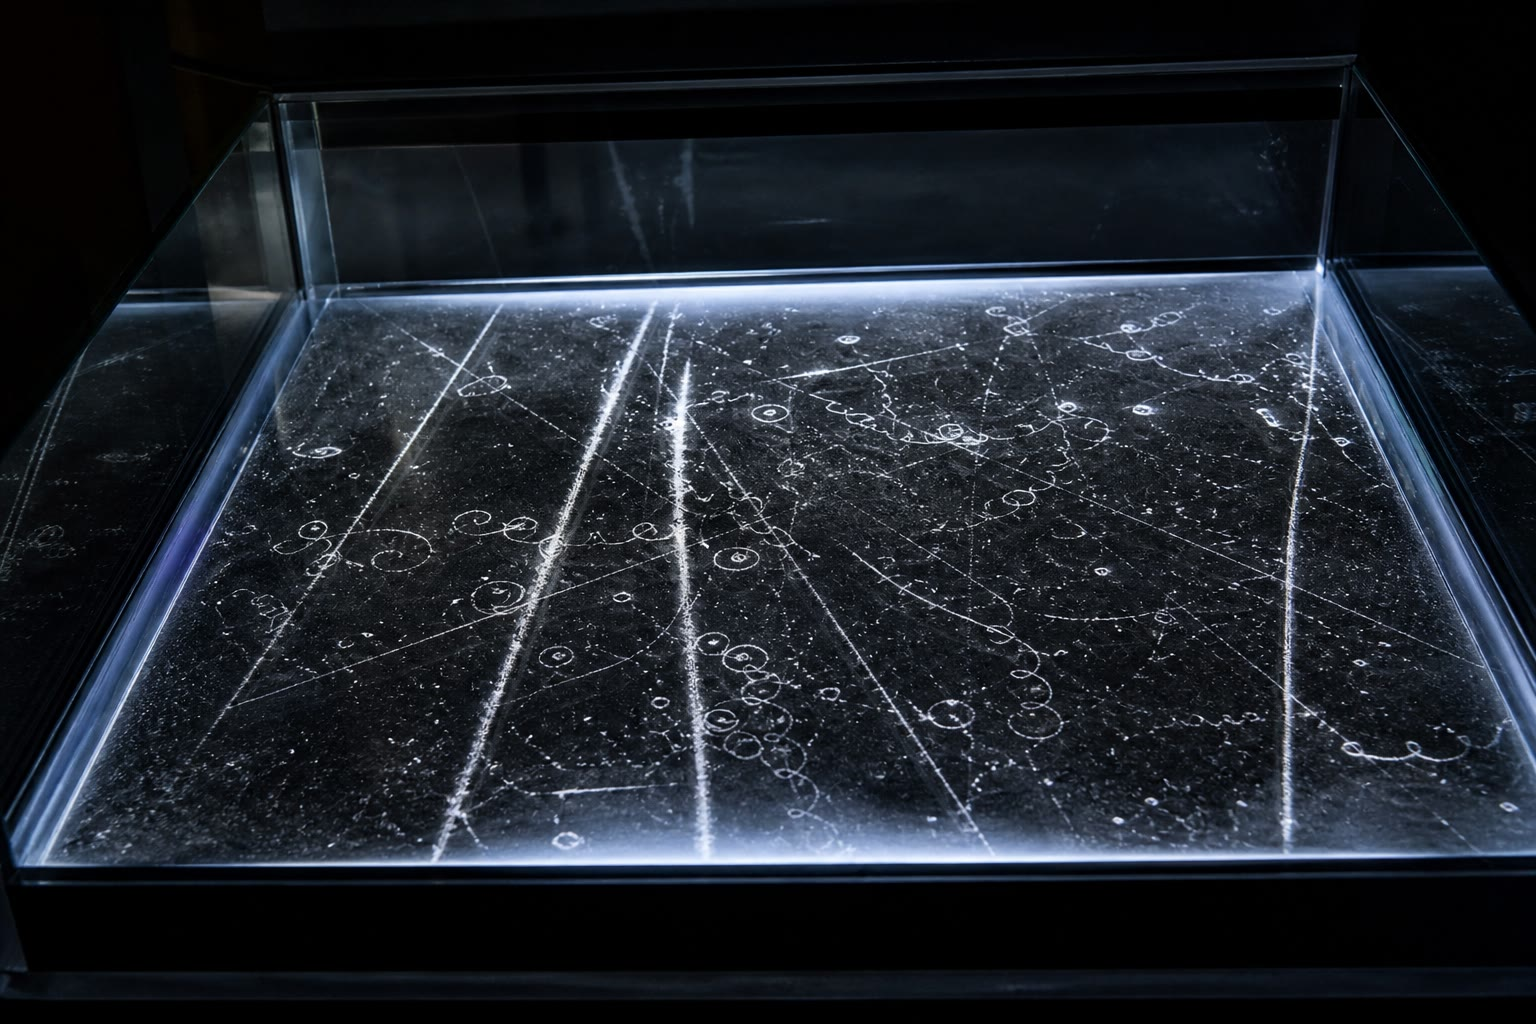
\includegraphics[width=0.58\linewidth]{images/book5/ai/b5-05-cloud-chamber.jpg}

{\small 带电粒子穿过云室。此类径迹——在磁场中弯曲、成对出现——使 $E = mc^2$ 从公式变为日常核算：正电子就是在这样一张照片上发现的。}
\end{omfigure}

\section{练习}

\begin{exercise}[$\star$]\label{exo:b3:relativistic-dynamics:1}
一个电子（$mc^2 = \qty{0.511}{MeV}$）以 $0.99c$ 运动。计算
$\gamma$、以 $\unit{MeV}/c$ 为单位的动量、总能量与
动能。对质子（$mc^2 = \qty{938}{MeV}$），
其动能为 \qty{1}{GeV}，提出同样的问题。
\end{exercise}

\begin{exercise}[$\star$]\label{exo:b3:relativistic-dynamics:2}
(a) 一克物质中沉睡着多少能量？(b) 广岛
爆炸释放了约 \qty{6e13}{J}：这对应多大的质量差？
(c) 太阳的辐射功率为 $L = \qty{3.8e26}{W}$：它每秒损失多少质量，
以及在一百亿年内，其 $\qty{2e30}{kg}$ 的质量损失了多大比例？
(d) 你的手机电池储存 \qty{5e4}{J} 的能量：
充满电的手机要重多少？
\end{exercise}

\begin{exercise}[$\star$]\label{exo:b3:relativistic-dynamics:3}
(a) 一支 \qty{5}{mW} 激光笔的光束每秒携带多少动量，
以及激光笔受到多大的力？(b) 太阳光（\qty{1.4}{kW/m^2}）
作用于理想反射的
\qty{100}{m^2} 太阳帆上的力多大？(c) 一个质量为 \qty{10}{kg} 的帆船，
从静止出发，经过一个月后速率多大？(d) 为什么彗星的尘埃尾
总是背离太阳？
\end{exercise}

\begin{exercise}[$\star$]\label{exo:b3:relativistic-dynamics:4}
单位练习。(a) 证明 $\unit{MeV}/c^2$ 是质量单位，
并将电子质量换算为千克。(b) 求
\qty{1}{GeV/c} 以 $\unit{kg.m/s}$ 计为多少？(c) \omterm{def:b3:relativistic-dynamics:four-momentum}{不变质量}平方
为 $s = \qty{16}{GeV^2}$（取 $c = 1$ 单位）：对应的质心系能量是多少？
(d) 粒子物理学家为何取
$c = 1$，若要得到国际单位制下的数值，读者须重新代入什么？
\end{exercise}

\begin{exercise}[$\star\star$]\label{exo:b3:relativistic-dynamics:5}
伯托齐的电子动能分别为 $0.5$、$1$、$4.5$ 和
\qty{15}{MeV}。(a) 计算牛顿预言的 $v^2 = 2E_k/m$，
对各动能分别以 $c^2$ 为单位表示。(b) 计算相对论的 $v^2/c^2$。(c)
在 \qty{15}{MeV} 下飞越 \qty{8.4}{m} 的飞行时间：计时器读数为多少，
牛顿理论本应预言多少？(d) 电子的
能量也曾以量热法测量——即通过它们撞击时的
热量：这一步为何是本实验的真正要点？
\end{exercise}

\begin{exercise}[$\star\star$]\label{exo:b3:relativistic-dynamics:6}
带电 π 介子在静止时衰变：$\pi^+ \to \mu^+\nu$，$m_\pi c^2 =
\qty{139.6}{MeV}$，$m_\mu c^2 = \qty{105.7}{MeV}$，$m_\nu \approx 0$。
(a) 证明 $pc = (m_\pi^2 - m_\mu^2)c^4/2m_\pi c^2$，并求其数值。
(b) 求 μ 子的动能与速率。(c) 求中微子的能量。
(d) 若 π 介子以 $\gamma_\pi = 50$ 飞行，衰变所得 μ 子在实验室系中的最大与最小能量为多少
（分别对应向前与向后衰变）？
\end{exercise}

\begin{exercise}[$\star\star$]\label{exo:b3:relativistic-dynamics:7}
\omterm{def:b3:relativistic-dynamics:four-momentum}{不变质量}的应用。(a) 两个能量各为 \qty{200}{MeV} 的光子
以 $60^\circ$ 的夹角彼此飞行：求该光子对的\omterm{def:b3:relativistic-dynamics:four-momentum}{不变质量}。
(b) 中性 π 介子（$m_{\pi^0}c^2 = \qty{135}{MeV}$）衰变为两个
光子：该光子对的\omterm{def:b3:relativistic-dynamics:four-momentum}{不变质量}为多少，在
每个参考系中是否相同？(c) 解释实验如何通过
衰变产物\omterm{def:b3:relativistic-dynamics:four-momentum}{不变质量}分布中的凸起而“发现”一个粒子。(d)
两个能量相等的光子恰好平行飞行：\omterm{def:b3:relativistic-dynamics:four-momentum}{不变质量}为多少？
这对光束的静止参考系说明了什么？
\end{exercise}

\begin{exercise}[$\star\star$]\label{exo:b3:relativistic-dynamics:8}
大型强子对撞机（LHC）的数据核算（质子能量 $E = \qty{6.8}{TeV}$）。(a) 求 $\gamma$ 以及
速率亏损 $c - v$（取 $c - v \approx c/2\gamma^2$）。(b) 求
周长为 \qty{27}{km} 的环上的公转频率，以及
每秒绕行的圈数。(c) 质子数为 \num{3e14} 的一束流所储存的能量，
以千克 TNT 计（\qty{4.2e6}{J/kg}）。(d) 两束流动能的
质能当量（以微克计）——即将生成的物质。
\end{exercise}

\begin{exercise}[$\star\star$]\label{exo:b3:relativistic-dynamics:9}
对撞光子。(a) 证明真空中单个光子无论能量多高，都不能
衰变为一对电子–正电子（利用
不变量）。(b) 设一个光子与能量为 $\epsilon$ 的第二个光子迎面相撞，
证明产生电子对需要 $E\epsilon \ge (m_{\text{e}}c^2)^2$。(c) 一个
\qty{511}{keV} 的光子需要什么伙伴？能量为 \qty{50}{keV} 的 X 射线呢？
(d) 宇宙充满星光与宇宙微波背景，
由（b）可预言 TeV 能量的 $\gamma$ 射线
在星系际空间中能抵达多远？
\end{exercise}

\begin{exercise}[$\star\star\star$]\label{exo:b3:relativistic-dynamics:10}
用\omterm{def:b3:relativistic-dynamics:four-momentum}{四维动量}推导康普顿效应。一个波长为 $\lambda$ 的光子与一个
静止电子相碰，并以角度 $\theta$ 散射。(a) 写出
\omterm{def:b3:relativistic-dynamics:four-momentum}{四维动量}守恒，并分离出末态电子的
不变量。(b) 推导
\[
\lambda' - \lambda = \frac{h}{m_{\text{e}}c}\,(1 - \cos\theta) .
\]
(c) 计算 $h/m_{\text{e}}c$ 与最大波长位移；为何该效应
在可见光下不可察觉，而对 X 射线却具有决定性？(d)
康普顿 1923 年的测量确立了关于光的什么结论，
而光电效应未能确立？
\end{exercise}

\begin{exercise}[$\star\star\star$]\label{exo:b3:relativistic-dynamics:11}
宇宙射线能谱的末端。宇宙中弥漫着微波
光子，典型能量为 $\epsilon = \qty{6e-4}{eV}$。一个质子
能量为 $E$，与其迎面相碰时，可被激发到
$\Delta$ 共振（$m_\Delta c^2 = \qty{1232}{MeV}$），
每次碰撞都会损失能量。(a) 证明阈值条件近似为 $4E\epsilon =
(m_\Delta^2 - m_{\text{p}}^2)c^4$。(b) 计算阈值 $E$。
(c) 超过阈值后，宇宙对质子而言在某一距离
（约 \qty{100}{Mly}）以外即不透明：这对观测到的宇宙射线
能谱有何预言（格赖森–扎采平–库兹明截断）？(d) 能量为
$\qty{3e20}{eV}$ 的宇宙射线已被记录到——“我的天哪”粒子：
它们的存在对其源提出了什么要求？
\end{exercise}

\begin{exercise}[$\star\star\star$]\label{exo:b3:relativistic-dynamics:12}
光子火箭。一枚初始质量为 $m_{\text{i}}$ 的火箭，以准直光束的形式喷出其
尾气，并达到速率 $\beta c$。(a)
由始末两态的能量与动量守恒，证明
\[
\frac{m_{\text{i}}}{m_{\text{f}}} =
\sqrt{\frac{1 + \beta}{1 - \beta}} = \eu^{\varphi} ,
\]
即快度的指数——相对论版的齐奥尔科夫斯基方程，
取最优尾气时的形式。(b) 求
达到 $0.9c$ 所需的质量比为多少？若还要达到 $0.9c$ 并在目的地\emph{停下}，又为多少？(c) 光束
必须以某种方式产生：若正反物质湮灭效率完美，
每千克有效载荷需要多少千克反物质？
这里指单程 $0.9c$ 之旅。(d) 全世界的反质子产量
为每年纳克量级。请用一句话就光子火箭作出结论。
\end{exercise}

\begin{omfigure}
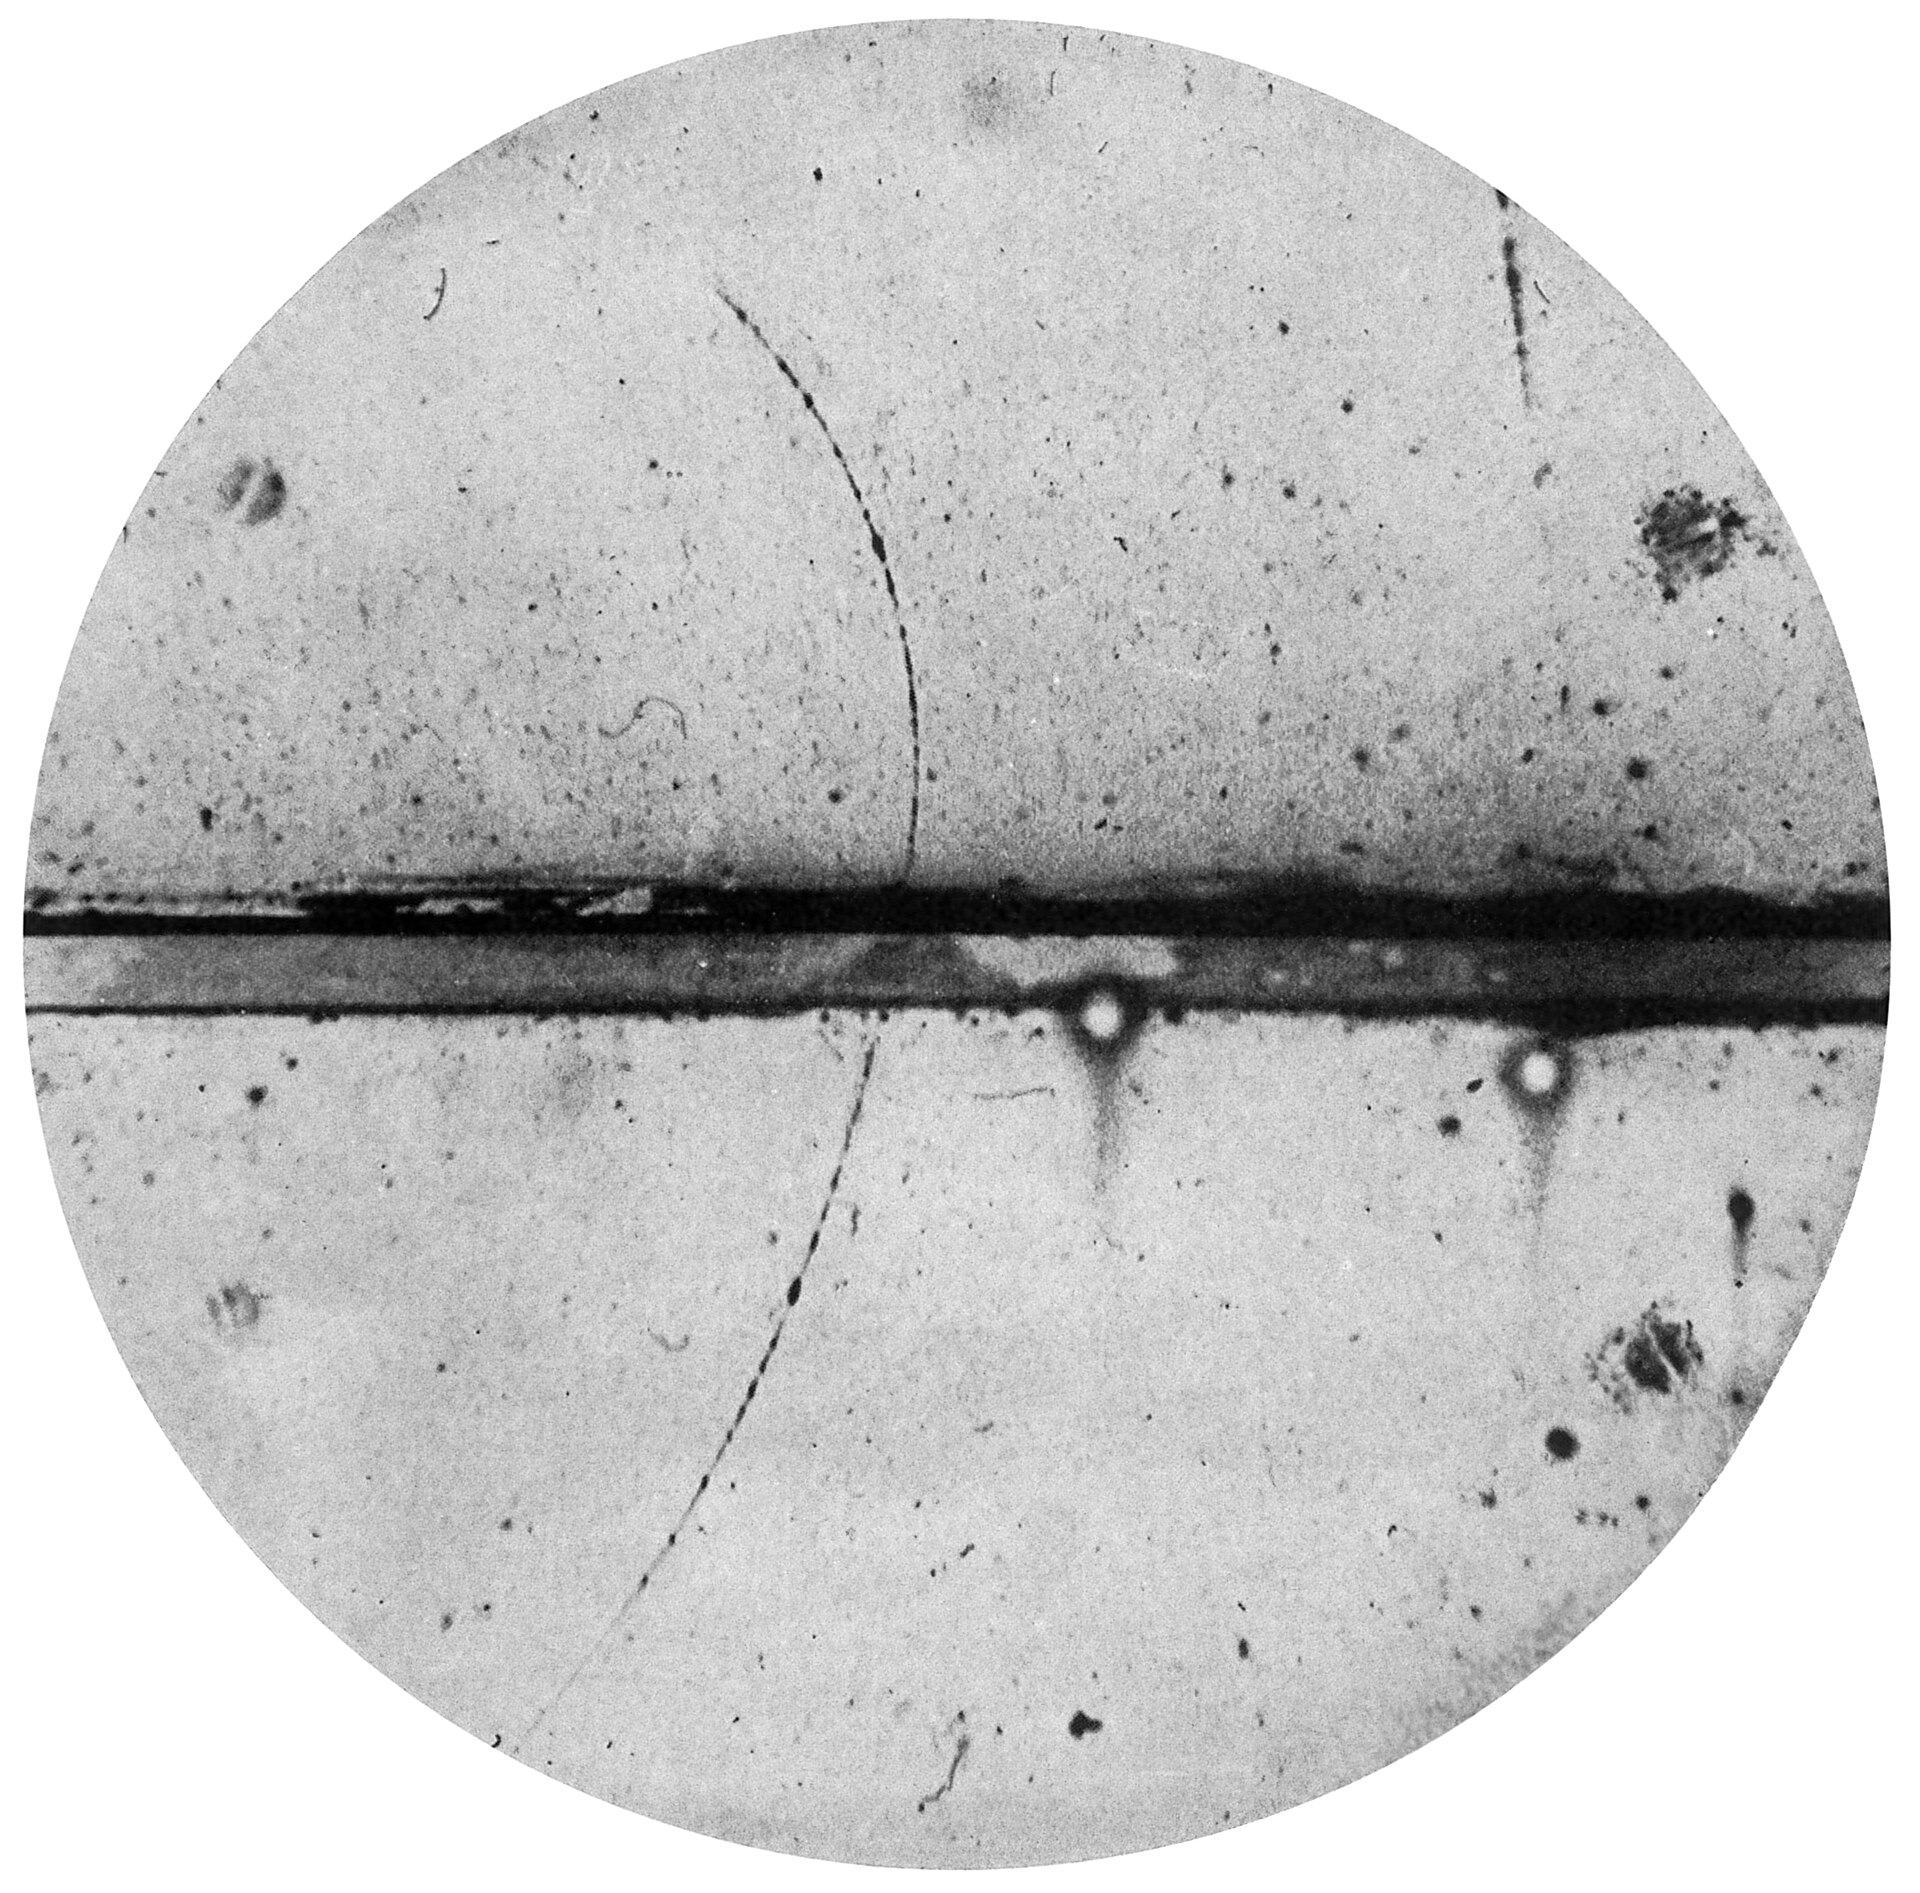
\includegraphics[width=0.5\linewidth]{images/book5/photo-positron-anderson.jpg}

{\small 反物质的发现（照片：Carl D. Anderson，1932 年，公有领域）：一个正电子穿过云室的铅板，向与电子相反的方向弯曲，弯曲程度又远大于质子应有的程度——$E = mc^2$ 的账目在此被反向验证。}
\end{omfigure}

\section{问题：制造物质——反质子与 Bevatron}

\begin{problem}[{周末问题——动量守恒如何
标定反世界的代价}]\label{pb:b3:relativistic-dynamics:1}
狄拉克方程自 1931 年起要求质子拥有一个
电荷相反的“镜像孪生”。制造它，意味着要用束流能量
去购买其\omterm{def:b3:relativistic-dynamics:momentum-energy}{静能}——动量守恒决定了这一价格。本题
将计算这一价格，设计付出此代价的机器，并追溯 1955 年的
发现。数据：$m_{\text{p}}c^2 = \qty{938.3}{MeV}$；电荷与
\emph{重子数}（质子与中子为 $+1$，反质子为 $-1$）
在每个反应中都守恒。

\medskip\noindent\textbf{第一部分——\omterm{def:b3:relativistic-dynamics:four-momentum}{四维动量}工具箱。}
\begin{enumerate}
  \item 对单个粒子证明 $E^2 - p^2c^2 = m^2c^4$，
        由 $E$ 与 $\vect p$ 的定义出发。
  \item 对于一个系统，为何 $E_{\text{总}}^2 -
        p_{\text{总}}^2c^2$ 在所有参考系中都相同？
        它在质心系中等于何值？
  \item 一束能量为 $E$ 的质子束轰击一个静止质子：证明
        $M^2c^4 = 2m_{\text{p}}^2c^4 + 2E\,m_{\text{p}}c^2$。
  \item 检验两个极限：低能时 $Mc^2 \to
        2m_{\text{p}}c^2$；高能时 $Mc^2 \approx
        \sqrt{2E\,m_{\text{p}}c^2}$——即平方根律。
  \item 仅当 $Mc^2$ 达到生成物静质量之和时，反应才被允许，
        且在阈值处，所有生成物在
        质心系中均静止。请论证
        这最后一条假设。
  \item 为何在固定靶的粒子产生中，生成物在实验室中的动能
        永远无法回收？
\end{enumerate}

\medskip\noindent\textbf{第二部分——标定反质子的价格。}
\begin{enumerate}[resume]
  \item 在 $p + p$ 碰撞中，产生反质子 $\bar p$ 的最廉价反应
        还须同时产生一个\emph{额外的}质子：
        写出该反应，并用电荷与重子数加以论证。
  \item 证明阈值要求 $Mc^2 = 4m_{\text{p}}c^2$。
  \item 推出所需束流能量 $E = 7m_{\text{p}}c^2$ 及
        动能 $T = 6m_{\text{p}}c^2$，并求 $T$ 的数值。
  \item 在阈值处，束流动能中实际转化为新静质量的
        比例是多少（其中 $2m_{\text{p}}c^2$ 为新增部分）？
        其余动能去了哪里？
  \item 在正面对撞的 $p$--$p$ 对撞机中，同一反应所需的
        \emph{每束}动能为多少？
        比较两种设计。
  \item 1954 年尚不存在对撞机（束流过于稀薄，无法彼此相碰）：
        是何种实际事实迫使人们选择固定靶方案，
        这在束流能量上付出了多大代价？
\end{enumerate}

\medskip\noindent\textbf{第三部分——设计 Bevatron。}
伯克利建成的这台机器达到了 $T = \qty{6.2}{GeV}$——
远高于阈值——其偶极磁场为 $B =
\qty{1.56}{T}$。
\begin{enumerate}[resume]
  \item 计算束流在最高能量下的总能量与动量。
  \item 计算偏转半径 $r = p/qB$，并与机器的
        \qty{15.2}{m} 作比较。
  \item 计算质子的速率，以及
        周长为 $2\pi r$ 的环上的绕行频率。
  \item 注入时质子动能为 \qty{10}{MeV}，计算其速率，
        并说明为何加速频率必须在每个周期内
        \emph{扫频}，
        （随 $E$ 增大，哪两个量会发生变化？）。
  \item 每圈获得约 \qty{1.5}{kV} 的能量，问需要多少圈，
        一个加速周期需要多长时间？
  \item 名称“Bevatron”来自 BeV，即十亿电子伏特。请用一行说明，
        是什么物理原因决定了设计数值 $6$
        及 BeV 的一个分数。
\end{enumerate}

\medskip\noindent\textbf{第四部分——1955 年的发现。}
\begin{enumerate}[resume]
  \item 磁铁使每个候选粒子沿圆周弯转：解释为何这一方式
        按\emph{动量}（$r = p/qB$）而非能量或速率挑选粒子，
        而按动量挑选的束流为何
        仍会混杂不同种类的粒子？
  \item 束流打在铜靶上，产生了大量负 π 介子
        （$m_\pi c^2 = \qty{139.6}{MeV}$），其中隐藏着少量反质子。
        谱仪选出了负电荷粒子，其动量为
        $p = \qty{1.19}{GeV}/c$，求该动量下
        反质子与 π 介子各自的速率。
  \item 沿 \qty{12}{m} 的飞行路径，计算两者的
        飞行时间：该发现需要怎样的时间分辨率？
  \item 第二个独立判据使用切伦科夫计数器，
        它只在速率超过阈值时才触发：安排哪种粒子
        去触发它，以及为何冗余验证对一项发现
        至关重要？
  \item 张伯伦与塞格雷统计到，约每 $\num{44000}$ 个 π 介子
        才出现一个反质子：为何阈值论证保证了即使高于阈值，
        计数率仍会极小？
  \item 反质子最终会与一个质子相遇并湮灭：
        每次事件释放多少能量，
        通常又转化为何种粒子？
  \item 概括这一著名结果：\omterm{def:b3:relativistic-dynamics:four-momentum}{四维动量}守恒在固定靶上将反质子的
        价格标定为 $T = 6m_{\text{p}}c^2 =
        \qty{5.6}{GeV}$；一台 \qty{6.2}{GeV}、
        \qty{15}{m} 的\omterm{prop:b3:relativistic-dynamics:force}{同步加速器}付出了这一代价，反世界
        由此成为实验室中的事实——即 1959 年诺贝尔奖。
\end{enumerate}
\end{problem}
